\documentclass{beamer}
\usepackage[T1]{polski}
\usepackage[polish]{babel}
\usepackage[utf8]{inputenc}
\usepackage[T1]{fontenc}
\usepackage[mediumspace,mediumqspace,Grey,squaren]{SIunits}
\usepackage{graphicx}
\usepackage{filecontents}

%\addbibresource{bibliography.bib}

%\setbeamertemplate{bibliography item}{\insertbiblabel}


\graphicspath{ {images/} }

\begin{document}
\title{Interfejsy wymiany danych}   
\bibliographystyle{plain}
\author{Jakub Postępski} 
\date{\today}

\frame{\titlepage} 


\section{Wstęp}

\frame{
	\frametitle{Systemy czasu rzeczywistego}
	Urządzenie techniczne, którego wynik i efekt działania jest zależny od chwili wypracowania tego wyniku. \cite{wiki:RTC}\\
	\vspace{1in}
	Systemy dzielimy na:
	\begin{itemize}
		\item Twarde
		\item Sztywne
		\item Miękkie
	\end{itemize}
}

\frame{
	\frametitle{Budowa ogólna}
	\begin{itemize}
		\item Fizyczne urządzenia i magistrale
		\item Algorytmy transportu danych
		\item Sterownik systemu operacyjnego
		\item Aplikacja
	\end{itemize}
}


\section{Warstwa fizyczna}
\frame{
	\frametitle{Przepustowośc}
	In computing, bandwidth is the bit-rate of available or consumed information capacity expressed typically in metric multiples of bits per second. Variously, bandwidth may be characterized as network bandwidth, data bandwidth, or digital bandwidth. \cite{wiki:Przepustowosc}
	\\Zależy od jakości ośrodka, w tym:
	\begin{itemize}
		\item Błędy transmisji
		\item Korekcja błędów
		\item Enkapsulacja
		\item Kolizje
		\item Kompresja
	\end{itemize}
}

\frame{
	\frametitle{Rodzaje łącz}
	\begin{itemize}
		\item Analogowe
		\item Cyfrowe
		\item Ze zwielokrotnieniem falowym
	\end{itemize}
	\begin{itemize}
		\item Szeregowe
		\item Równoległe
	\end{itemize}
}

\frame{
	\frametitle{Otwarty kolektor}
	\begin{figure}
	\centering
	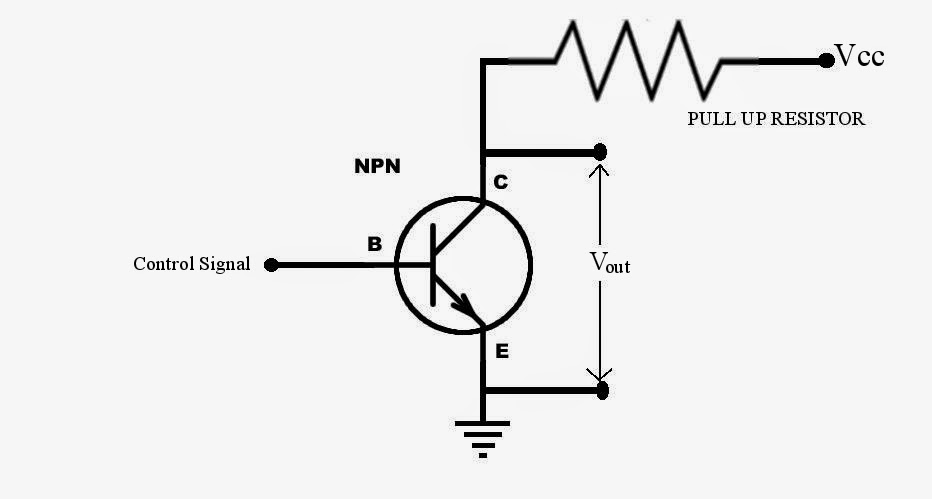
\includegraphics[width=0.9\linewidth]{open_collector}
	\caption{Schemat otwartego kolekotra\cite{image:collector}}
	\label{fig:open_collector}
	\end{figure}
}
\frame{
	\frametitle{Para różnicowa}
	\begin{figure}
		\centering
		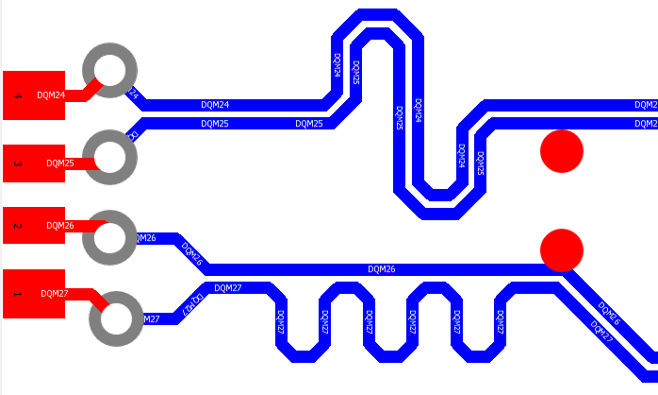
\includegraphics[width=0.9\linewidth]{differential}
		\caption{Przykładowa realizacja pary różnicowej na PCB\cite{image:collector}}
		\label{fig:differential}
	\end{figure}
}
\frame{
	\frametitle{Magistrale szeregowe i równoległe}
}

\subsection{Światłowody}
\frame{
	\frametitle{Światłowody}
	\begin{itemize}
		\item Małe tłumienie
		\item Brak zakłóceń elektromagnetycznych
		\item Problemy z fizycznymi połączeniami
	\end{itemize}
	\begin{itemize}
		\item Wielomodowe
		\item Jednomodowe
	\end{itemize}
}


\frame{
	\frametitle{CAN}
	
}

\frame{
	\frametitle{USB}
}

\frame{
	\frametitle{SPI}
}


\frame{
	\frametitle{UART}	
}


\frame{
	\frametitle{RS-232}	
}

\frame{
	\frametitle{I$^2$C}
}


\frame{
	\frametitle{Ethernet - kable miedziane}
	\begin{itemize}
		\item Złącze 8P8C
		\item Topologia gwiazdy
		\item Połaczenia proste pomiędzy switchami i komputerami
		\item Połączenia krosowane pomiędzy dwoma switchami lub dwoma komputerami
		\item Odległość transmisji wynosi 100 m
		
	\end{itemize}
	
}

\section{Warstwa transportu danych}

\frame{
	\frametitle{Modbus}
}

\frame{
	\frametitle{CANOpen}
}

\frame{
	\frametitle{Ethercat}	
}

\frame{
	\frametitle{Gigavision}	
}


\section{Przykłady praktyczne}
\frame{
	\frametitle{Mała szklarnia}	
}

\frame{
	\frametitle{Serwonapęd}	
}

\frame{
	\frametitle{Czujnik siły}	
}

\frame{
	\frametitle{Robot mobilny}
}

\frame{
	\frametitle{Kontrola trakcji elektrycznej lub kolejowej}	
}
\frame{
	\frametitle{Kamera HD}	
}

\section{Podsumowanie}
\frame{
	\frametitle{Literatura}
	\bibliography{bibliography}
}

\frame{
	}
\end{document}
